%!TEX root = uist14.tex
\section{Introduction}

%% from the swarm vision to the necessity of selection
Increasingly, objects in our built environment are equipped with computation and communication, making them potential targets for user interaction. 
%Such interactions might be {\em explicit} -- controlling smart appliances such as intelligent lighting, AV equipment, or HVAC systems; or {\em implicit} -- tracking the user's attention to gauge interest e.g., for targeted-advertisement or context-aware computing \bjoern{second part needs to be stronger}. 
To initiate such interaction requires {\em selection} information by which a system keeps track of the user's {\em locus of attention}~\cite{raskin} in the world.

%% previous approaches are limited
Past research has introduced techniques of augmenting hand-held mobile devices with accessories like laser pointers to enable direct aiming at target devices in space~\cite{beigl_point_1999,patel_2-way_2003}. While promising, some drawbacks of using handheld devices are that the device first has to be retrieved (e.g., from a pocket) and consciously aimed; that the user's hands are required to be free for operation (one to hold the device, one to operate the touch screen or keyboard); and that the user's visual attention is now split between looking down at a screen and out at targets in the world. 

\begin{figure}[t]
\centering
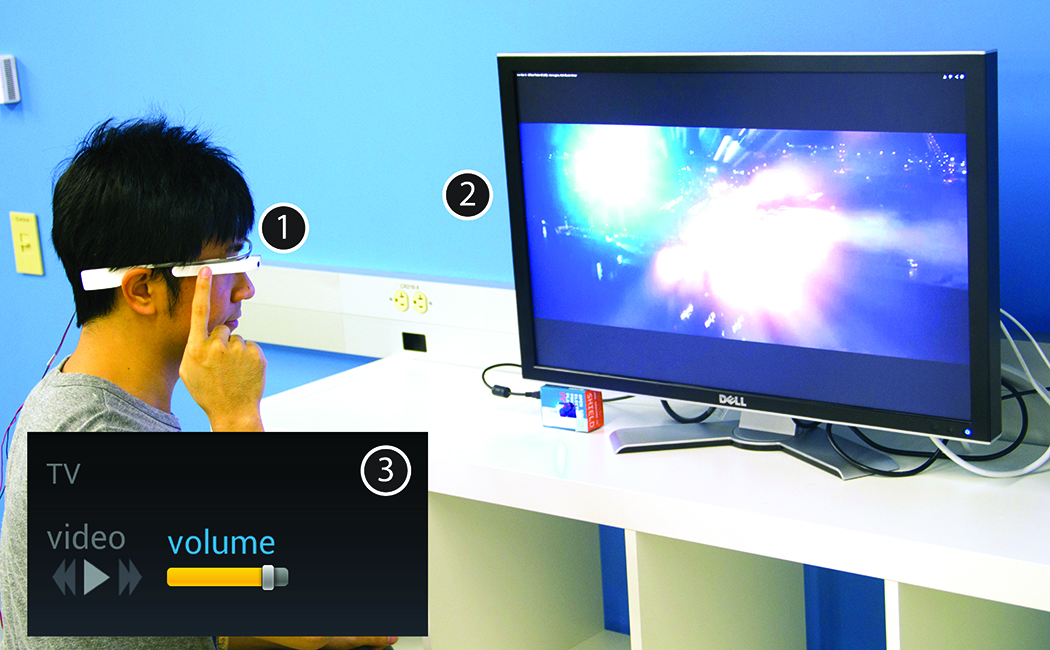
\includegraphics[width=1.0\columnwidth]{figures/teaser.jpg}
\caption{An example application of head-orientation targeting: Using an augmented head-worn device (1), users can control smart home appliances (2) by looking at them. A near-eye display then shows an appliance control UI (3), which users navigate through multitouch gestures.}
\label{fig:teaser}
\end{figure}

%% introducing head-worn computing and head orientation
Emerging head-worn computing devices have the potential to overcome some of these limitations: because they are worn, they do not require retrieval; they may enable hands-free or uni-manual interactions; and they offer near-eye or see-through displays to present information adjacent to physical objects in the wearer's field of view. We thus investigate the research question how such computing devices may be used for selection of physical targets in space.

Because they are head-worn, such devices can naturally exploit the user's head orientation, an important, but also imprecise indicator of the user's locus of attention: it contains the general direction, but not the particular point of focus. While gaze tracking could provide further information about a user's focus, when operating in unconstrained environments, translating gaze information into identification and selection of an object is an open problem.
We therefore study how to leverage head-orientation alone for target selection in physical spaces. 

The imprecision of human head movement suggests adapting area cursor techniques known from assistive devices~\cite{kabbash1995prince,worden1997making,Findlater-uist2010}. Such techniques employ a two-step selection process: {\em coarse} selection of an area of interest, followed by {\em refinement} to select a target within that region.

We propose an area-selection technique that can be readily implemented with small hardware changes to emerging wearable devices. We augment Google Glass\footnote{\url{http://www.google.com/glass/start/}} to enable (IR) communication between Glass and target appliances. The cone shape of light emitted by an IR LED (a diameter of 60-120cm and distance up to 6m) provides the {\em coarse} selection area. To {\em refine} selection when multiple targets have received IR signals, we introduce three different disambiguation techniques. First, targets compare received IR signal intensity to make a default selection among signal recipients. Second, we use IR intensity changes from head movement to switch between signal recipients when a user explicitly enters a refinement quasi-mode. Third, we always leave the option of manually changing the current targets through explicit list navigation.
%% three ways

We also contribute empirical data on the system performance, usability, and user experience of head-orientation targeting and device control. We first report measurements of range and beam characteristics of our controller. We then conduct a study with $14$ participants that compares acquisition times for physical targets in a room for our technique and an alternative list selection interface. We find that target acquisition through head orientation is preferred by users and is faster than list selection, given the constraints of linear input using a head-worn touch controller. 
We then quantify the additional benefit of using IR-intensity disambiguation \bjoern{and find XYZ.}. \bjoern{Say something about the inferred map if we get around to it}.

%---
We also demonstrate and example application of our technique for a remote control of smart appliances: a user looks at the appliance she wishes to control and confirms selection by tapping - an appliance-specific user interface is then shown on the user's near-eye display.

%Orientation-based selection enables a wide range of context-aware applications. Examples include smart home remote control, break reminder monitor starer, museum attention tracking, indoor positioning, etc. In Figure\,\ref{fig:teaser}, it's a demonstration of the ``universal remote control'' scenario. The user can easily select the smart appliances by simply looking at it's general direction and confirm such selection with either voice command or by tapping the Glass input pad. Then an appliance-specific control UI will be shown on the head-mounted display. For this application, we have asked 14 participants to try the system and we report the qualitative results from them performing home automation tasks.



%% Contribution
In summary, this paper makes the following contributions:
\begin{itemize}
\item We design and implement a novel head-orientation based selection technique for physical targets based on IR communication. We introduce disambiguation techniques to address the inherent imprecision of head orientation.
\item We present evaluations that compare head orientation targeting to list selection and quantify the benefits of automatic disambiguation.
\item We demonstrate a home appliance remote control application built on top of our selection technique.
\end{itemize}

%\ben{Having problem fixing the reference}.\bjoern{skip this - we want to be brief.}
%In the remainder of this paper, we will first describe the related works in physical selection and targeting. Given that we focus our scope on head orientation, in Section~\ref{sec:background} we will briefly review human's neck ergonomics as the background for head orientation. In Section~\ref{sec:syst-design-prot}, we then present our system designed for the study of head orientation based selection. The prototype is also what we have used for building the example applications. The disambiguation techniques are discussed in Section~\ref{sec:disamb-techn}, which is followed by the study and evaluation in Section~\ref{sec:evaluation}. To further show the usefulness of having such head orientation-based selection, we describe the enabled applications in Section~\ref{sec:applications}, with detailed implementation about the ``universal remote control'' application. The discussion and conclusion are in Section~\ref{sec:discussion} and Section~\ref{sec:conclusion} respectively. 

%%% Local Variables: 
%%% mode: latex
%%% TeX-master: "uist14"
%%% End: 
